\subsection{Bewertung verschiedener DFT-Größen}\label{sec:AnalyseBewertungTwiddlefaktornMatrizen}

In der Tabelle \ref{tab:DFT-TwiddlefaktorMatrizenBewertung} werden die DFT-Matrizen einander gegenüber gestellt.
Anders als die \gls{dct} haben die Twiddlefaktormatrix und deshalb auch das Ergebnis der \gls{dft} einen Real- und einen Imaginärteil.
Die Beurteilung basiert auf dem Matlab-Skript aus Anhang \ref{src:dft_bewertung}. 
Wie zu sehen ist, schneiden vor allem die 8x8- und die 12x12-DFT gut ab. Da letztere nur zum Vergleich mit aufgenommen wurde, ist die 
8x8-DFT der klare Favorit, welcher im folgenden Abschnitt genauer betrachtet werden soll.


 \vspace{1cm}
 \begingroup
  \renewcommand*{\arraystretch}{1.2} % Zeilenabstand der Tabelle
  \begin{table}[!ht]
  \centering
  \caption{Bewertung der DFT-Twiddlefaktor-Matrizen}
   \begin{tabular}{lccccc}
   \hline
    N							& 8	& 9	& 12	& 15		& 16 \\
    \hline
    N$\times$N						& 64	& 81	& 144	& 225		& 256 \\
    \rowcolor{lightgray}
    trivial $\Re$ 					& 48	& 45	& 128	& 81		& 128 \\
    \rowcolor{lightgray}
    nicht triv. $\Re$					& 16	& 36	& 16	& 144		& 128 \\
    triv. $\Im$ 					& 48	& 21	& 96	& 45		& 128 \\
    nicht triv. $\Im$ 					& 16	& 60	& 48	& 180		& 128 \\
    \rowcolor{lightgray}
    $\sum$ triv. 					& 96	& 66	& 224	& 126		& 256 \\
    \rowcolor{lightgray}
    $\sum$ nicht triv. 					& 32	& 96	& 64	& 324		& 256 \\
    Anzahl verschiedener nicht trivialer Werte          & 1     & 7     & 1     & 13            & 3 \\
    Verhältnis  $\sum$ trivial / $\sum$ nicht trivial	& 3	& 0,6875& 3,5	& 0,3889	& 1\\
    \hline
   \end{tabular}
   \label{tab:DFT-TwiddlefaktorMatrizenBewertung}
  \end{table}
 \endgroup
 \vspace{1cm}
 
 
 \section{Genauere Betrachtung der 8x8-DFT}
 In Grafik \ref{pic:Einheitskreis_Faktoren} sind die Twiddlefaktoren der 8x8-DFT im Einheitskreis dargestellt. 
 Betragsmäßig treten die Werte 0, 1 und  $\nicefrac{\sqrt{2}}{2}$ auf. Gemäß der obigen Definition für nicht triviale Werte zählt ausschließlich der letztgenannte zu diesen.
 Eine besondere Eigenschaft ist, dass für nicht triviale Multiplikationen Real- und Imaginärteil zumindest vom Betrag her identisch sind.
 Dies liegt daran, dass
 der Einheitskreis in acht Teile geteilt wird und für beispielsweise $\frac{2\cdot\pi}{8}=\frac{\pi}{4}$ der Sinus- und Kosinuswert identisch sind. Darüber hinaus ist dies auch 
 der einzige Wert, der sowohl einen Real- aus auch einen Imaginärteil besitzt. Alle anderen Faktoren haben in einem von beiden Teilen $\abs{1}$ und somit im anderen Teil 0.
 Hieraus resultiert, dass die Hälfte der Berechnungen der nicht trivialen Werte, die für die reelle Matrix gemacht werden müssen,
 direkt für den imaginären Anteil übernommen werden könnten. Die andere Hälfte müsste lediglich negiert werden. 
 Deshalb kann das berechnete Verhältnis von 3 in Tabelle \ref{tab:DFT-TwiddlefaktorMatrizenBewertung} als deutlich höher angenommen werden.
 
 Anfangs wurde in Betracht gezogen das 1er-Komplement zu verwenden, da hierbei zwei betragsmäßig identische Zahen sich nur durch ihr höchstwertigstes 
 Bit unterscheiden. Auf diese Weise könnte das selbe Resultat für den Imaginär- wie für den Realteil verwendet werden, das Vorzeichen würde sich über eine 
 einfache XOR-Verknüpfung beider MSB der Multiplikanden ergeben.
 Diesem Vorteil steht jedoch eine aufwändigere Subtraktion (bzw. Addition negativer Zahlen) gegenüber. Der zusätzliche Aufwand entspricht 
 etwa dem der Bildung des 2er-Komplements. Aus diesem Grund und da das 2er-Komplement deutlich verbreiteter ist sowie weitere Vorteile bringt wie 
 beispielsweise keine Doppeldeutigkeit durch eine negative Null hat, wurde sich hierfür entschieden.
 
 
 In späteren Analysen konnte festgestellt werden, dass sowohl für den Real- als auch den Imaginärteil gleichviele Multiplikationen mit positiven wie mit negativen Faktoren 
 durchgefürht werden müssen. Dies lässt sich anhand des Einheitskreises in Abb. \ref{pic:Einheitskreis_Faktoren} und der Abbildung \ref{pic:Twiddlefaktoren_Darstellung8x8}
 nachvollziehen. Aus Abschnitt \ref{sec:Matrixmultiplikation} ist bekannt, dass bei einer Matrixmultiplikation Elemente multipliziert und anschließend die Ergebnisse 
 aufsummiert. Da es das Kommutativgesetz erlaubt die berechneten Ergebnisse auch in einer anderen Reihenfolge zu addieren, 
 
 In Abbildung \ref{pic:Twiddlefaktoren_Darstellung8x8} sind zur besseren Veranschaulichung die komplexen Zeiger der Twiddlefaktoren dargestellt. Sie sind aufgeteilt auf 8 
 Einheitskreise, wobei jeder einen Laufindex ($m$) des Zeitbereichs abdeckt. In den einzelnen Kreisen sind wiederum alle Laufindizes ($n$) des Frequenzbereichs zu sehen.
  
 In Abbildung \ref{pic:MatrizenDarstellungTwiddlefaktoren} ist zu sehen, dass die 2., 4., 6., und 8. Zeile je vier nicht triviale und komplexe Faktoren enthält. 
 Darüber hinaus ist ersichtlich, dass für komplexe Eingangswerte in den genannten Zeilen 12 und in den übrigen 8 Multiplikationen erfolgen müssen. Dies kann anhand der 
 Gleichungen (\ref{eq:komplexe_Multiplikation}) und (\ref{eq:halb_komplexe_Multiplikation}) nachvollzogen werden.
 Das lässt sich ausnutzen, um keine Negationen der Eingangs- und Zwischenwerte durchführen zu müssen. 
 
 \begin{align}\label{eq:halb_komplexe_Multiplikation}
\begin{split}
 e + jf &= a \cdot (c + jd)\\
        &= a \cdot c + j(a \cdot d)\\
\end{split}
\end{align}
 
 
 
 Darüber hinaus
 minimiert sich bei geschickter Anordnung das Risiko eines Überlaufs. Wie in Abschnitt \ref{sec:NumerischeUngenauigkeiten} erwähnt, ist dies nicht Gegenstand dieser Arbeit,
 weshalb der Einfachheit wegen zur Sicherheit dennoch nach jeder Addition oder Subtraktion das Ergebnis durch einen Bitshift halbiert wird. 
 Es sei an dieser Stelle lediglich angemerkt, dass über die Eingangswerte die Annahme getroffen werden kann, dass aufeinanderfolgende Werte das selbe Vorzeichen haben. 
 Dies ließe sich ausnutzen, um noch weiter die Wahrscheinlichkeit zu reduzieren, dass es zu einem Überlauf kommt. 


 \begin{figure}[!t]
  \centering
  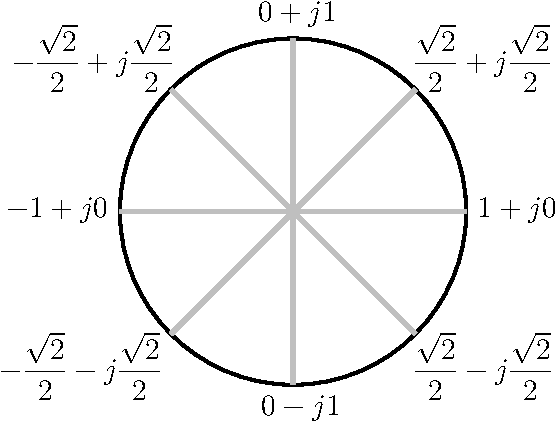
\includegraphics[width=0.3\textwidth]{img/Einheitskreis-crop.pdf}
  \caption{Einheitskreis mit relevanten Werten der 8x8-DFT}
  \label{pic:Einheitskreis_Faktoren}
\end{figure}
  
 


\begin{figure}[!ht]
 \centering
 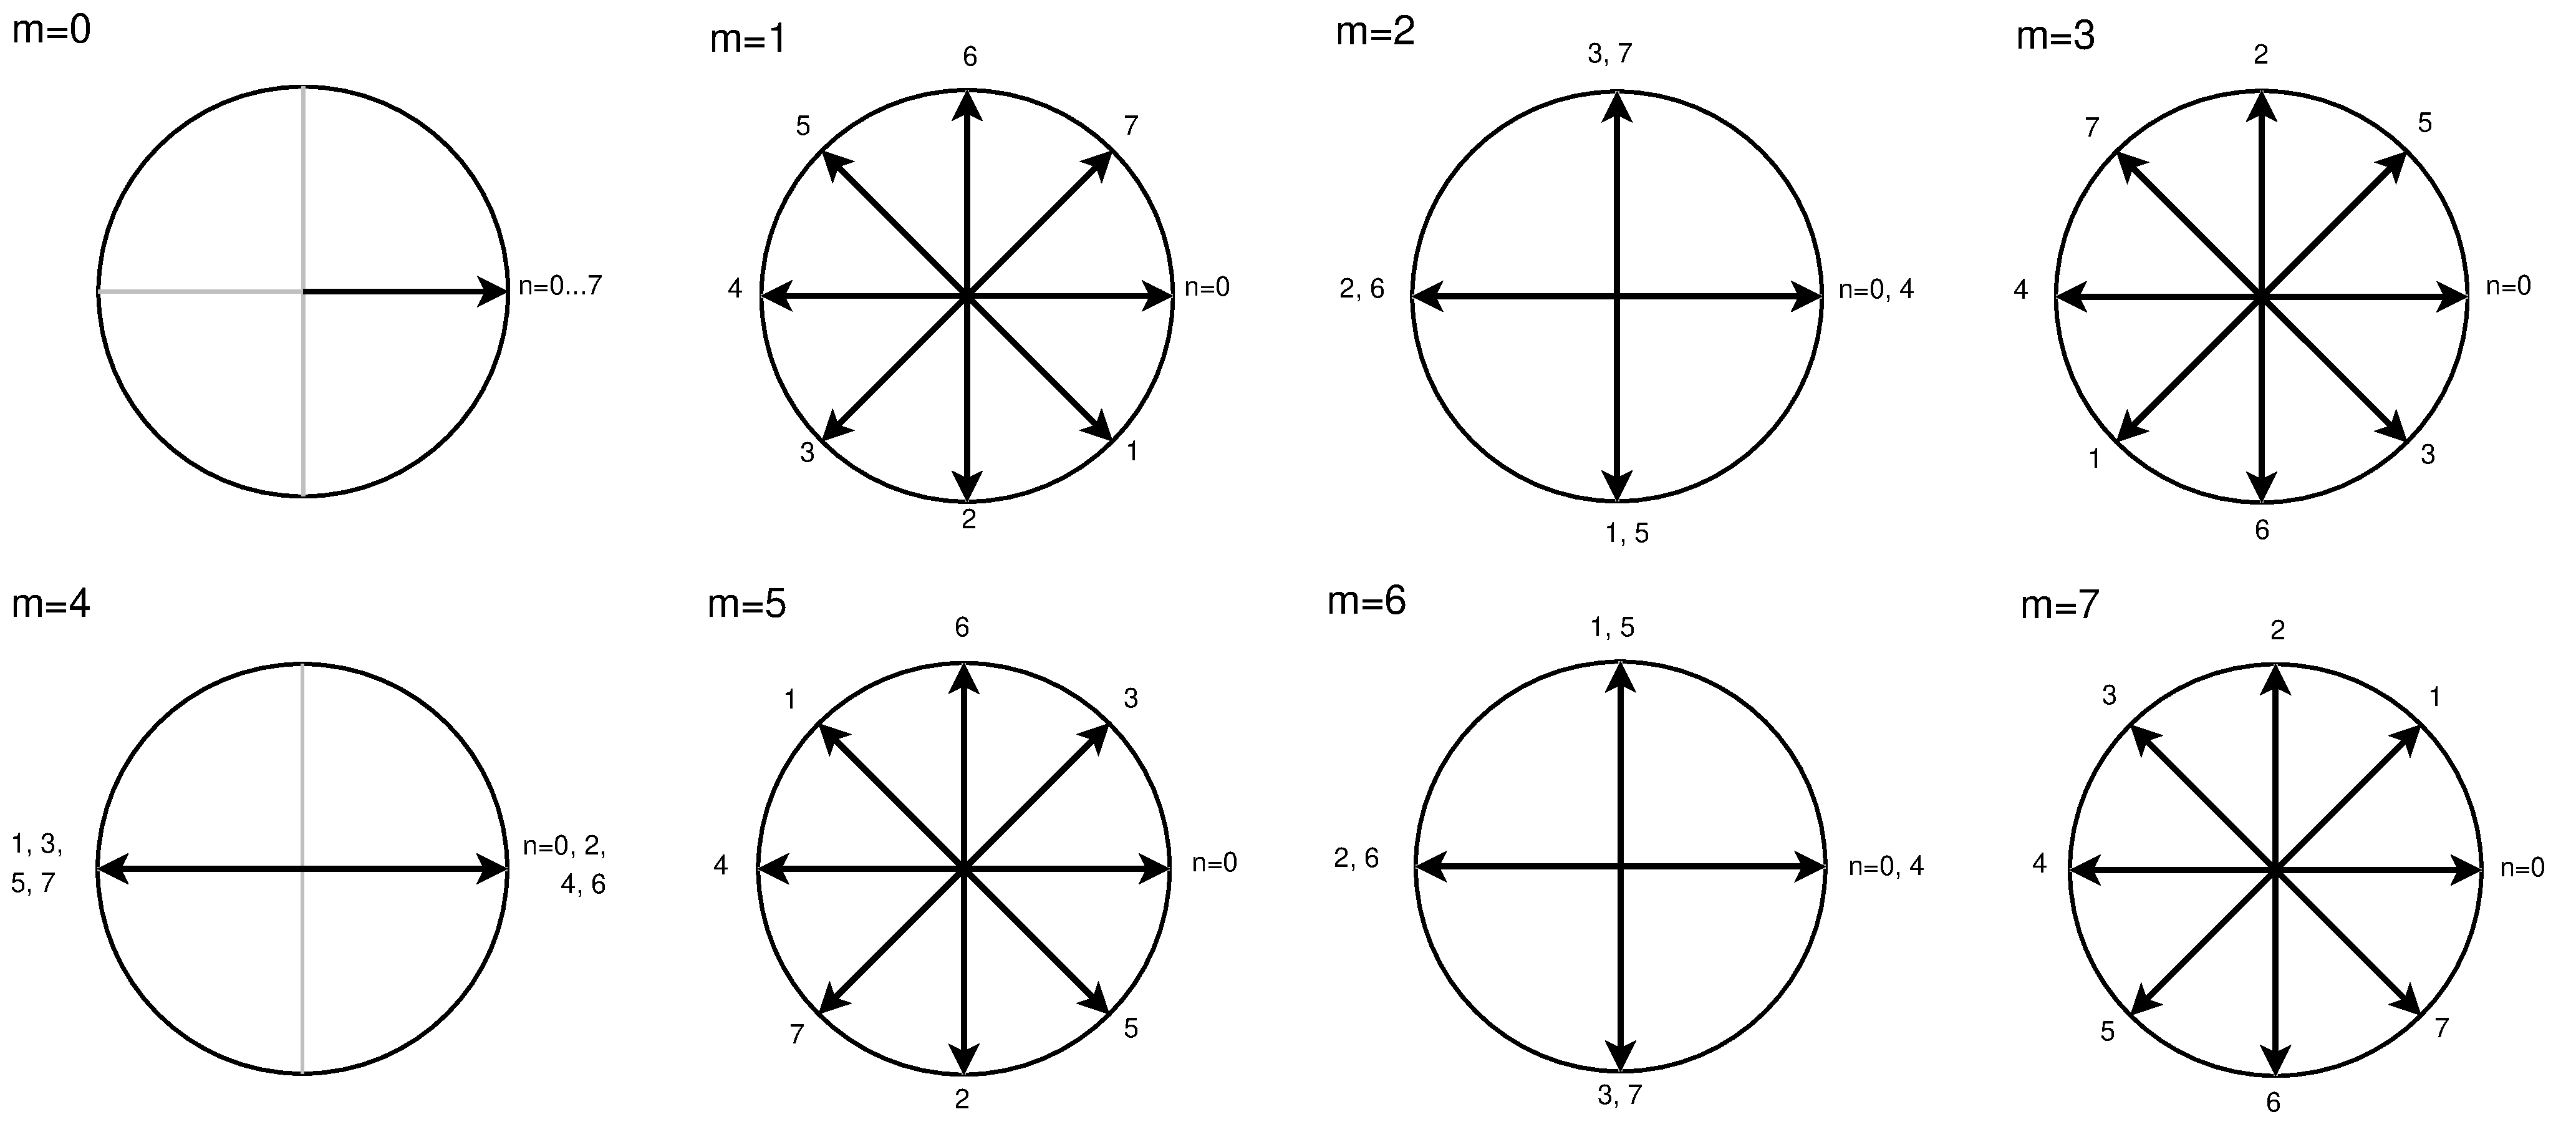
\includegraphics[width=1\textwidth]{img/Twiddlefaktoren_Einheitskreis.eps}
 \caption{Twiddlefaktoren der 8$\times$8-Matrix, aufgeteilt auf die Laufindizes $m$ und $n$. $m$ bezieht sich auf das Element im Ausgangsvektor $\vec{X}$, $n$ auf den Eingangsvektor $\vec{x}$. Siehe auch Gl. (\ref{eq:dft}) }
 \label{pic:Twiddlefaktoren_Darstellung8x8}
\end{figure}

\vspace{0.5cm}


 

\begin{minipage}{0.9\textwidth}
\begingroup
 \renewcommand*{\arraystretch}{0.95} % Zeilenabstand der Tabelle

\begin{center}
  \[
   \stackrel{\mbox{$Re\{W\}$}}{
    \begin{bmatrix}
     \myboxOnePos 	& \myboxOnePos 		& \myboxOnePos 	& \myboxOnePos 		& \myboxOnePos 	& \myboxOnePos 		& \myboxOnePos 	& \myboxOnePos \\
     \myboxOnePos 	& \myboxSqrtPos 	& \myboxZero 	& \myboxSqrtNeg		& \myboxOneNeg	& \myboxSqrtNeg		& \myboxZero	& \myboxSqrtPos \\
     \myboxOnePos 	& \myboxZero 		& \myboxOneNeg 	& \myboxZero 		& \myboxOnePos 	& \myboxZero 		& \myboxOneNeg 	& \myboxZero \\
     \myboxOnePos 	& \myboxSqrtNeg 	& \myboxZero 	& \myboxSqrtPos 	& \myboxOneNeg 	& \myboxSqrtPos 	& \myboxZero 	& \myboxSqrtNeg \\
     \myboxOnePos 	& \myboxOneNeg 		& \myboxOnePos 	& \myboxOneNeg 		& \myboxOnePos 	& \myboxOneNeg 		& \myboxOnePos 	& \myboxOneNeg \\
     \myboxOnePos 	& \myboxSqrtNeg 	& \myboxZero 	& \myboxSqrtPos 	& \myboxOneNeg 	& \myboxSqrtPos 	& \myboxZero 	& \myboxSqrtNeg \\
     \myboxOnePos 	& \myboxZero 		& \myboxOneNeg 	& \myboxZero 		& \myboxOnePos 	& \myboxZero 		& \myboxOneNeg 	& \myboxZero \\
     \myboxOnePos 	& \myboxSqrtPos 	& \myboxZero 	& \myboxSqrtNeg		& \myboxOneNeg	& \myboxSqrtNeg		& \myboxZero	& \myboxSqrtPos 
    \end{bmatrix}
   }
   \hspace{1cm}
   \stackrel{\mbox{$Im\{W\}$}}{
    \begin{bmatrix}
     \myboxZero 	& \myboxZero 		& \myboxZero 	& \myboxZero 		& \myboxZero 	& \myboxZero 		& \myboxZero 	& \myboxZero \\
     \myboxZero 	& \myboxSqrtNeg 	& \myboxOneNeg 	& \myboxSqrtNeg		& \myboxZero	& \myboxSqrtPos		& \myboxOnePos	& \myboxSqrtPos \\
     \myboxZero 	& \myboxOneNeg 		& \myboxZero 	& \myboxOnePos 		& \myboxZero 	& \myboxOneNeg 		& \myboxZero 	& \myboxOnePos \\
     \myboxZero 	& \myboxSqrtNeg 	& \myboxOnePos 	& \myboxSqrtNeg 	& \myboxZero 	& \myboxSqrtPos 	& \myboxOneNeg 	& \myboxSqrtPos \\
     \myboxZero 	& \myboxZero 		& \myboxZero 	& \myboxZero 		& \myboxZero 	& \myboxZero 		& \myboxZero 	& \myboxZero \\
     \myboxZero 	& \myboxSqrtPos 	& \myboxOneNeg 	& \myboxSqrtPos		& \myboxZero 	& \myboxSqrtNeg 	& \myboxOnePos 	& \myboxSqrtNeg \\
     \myboxZero 	& \myboxOnePos 		& \myboxZero 	& \myboxOneNeg 		& \myboxZero 	& \myboxOnePos 		& \myboxZero 	& \myboxOneNeg \\
     \myboxZero 	& \myboxSqrtPos 	& \myboxOnePos 	& \myboxSqrtPos		& \myboxZero	& \myboxSqrtNeg		& \myboxOneNeg	& \myboxSqrtNeg 
    \end{bmatrix}
   }
  \]
\vspace{0.5cm}
  Legende: $\myboxOnePos$ = 1 \quad $\myboxOneNeg$ = -1 \quad $\myboxZero$ = 0 \quad $\myboxSqrtPos$ = $\nicefrac{\sqrt{2}}{2}$ \quad $\myboxSqrtNeg$ = -$\nicefrac{\sqrt{2}}{2}$
  \captionof{figure}{Matrix-Darstellung der 8x8-DFT-Twiddlefaktoren aufgeteilt nach Real- und Imaginärteil}
  \label{pic:MatrizenDarstellungTwiddlefaktoren}
\end{center}
\endgroup
\end{minipage}


\vspace{0.5cm}


Sowohl der Abbildung \ref{pic:Twiddlefaktoren_Darstellung8x8} als auch insbesondere der Darstellung \ref{pic:MatrizenDarstellungTwiddlefaktoren} lassen sich sehr gut die 
Symmetrien erkennen, die diese Twiddlefaktormatrix so vorteilhaft machen.
